\chapter{Power Supplies, Motors \& Pumps}\label{ch:motors}

\begin{tipbox}[When to Read This Chapter]
\textbf{Sprint~2--3}: Read when sizing motors, pumps, or power supplies for your design. The motor/driver quick-reference table and the belt conveyor worked example are the most immediately useful. \textbf{Sprint~3 (CDR)}: Verify your power budget using the battery sizing section. \textbf{Sprint~4}: Return to the motor driver section when wiring actuators.
\end{tipbox}


\vspace{1em}




\vspace{1em}

% ══════════════════════════════════════════════════════════════════════
\section{Power Supply Selection}
% ══════════════════════════════════════════════════════════════════════

\subsection{What a Power Supply Does}

A power supply converts electrical energy from a source, AC mains, battery, solar panel, or USB, into one or more regulated DC voltage rails that your circuits and actuators require. Every component in your design has a specific voltage and current requirement. A typical student project might need 3.3\,V for the microcontroller, 5\,V for sensors and logic, and 12\,V or 24\,V for motors and solenoids\index{solenoid}. The power supply must deliver all of these simultaneously with adequate regulation and current capacity.

\subsection{Linear Regulators (LDO)}

Linear regulators are the simplest power supply topology. They are essentially a controllable series resistance that drops the input voltage to the desired output, dissipating the excess as heat.

\begin{equation}
  P_{\text{waste}} = (V_{\text{in}} - V_{\text{out}}) \times I_{\text{load}}, \qquad \eta = \frac{V_{\text{out}}}{V_{\text{in}}} \times 100\%
\end{equation}

An LM7805 producing 5\,V from 12\,V at 1\,A wastes 7\,W as heat with only 42\% efficiency. A low-dropout (LDO) regulator reduces the minimum input-to-output voltage difference to as little as 200\,mV, improving efficiency when the differential is small.

\begin{tipbox}[When to Use an LDO]
Use LDOs when: (1) the voltage drop is small ($<2\,V$), (2) current is under $\sim$1\,A, (3) noise matters (analog sensors, audio, ADCs), or (4) simplicity matters (only 2 capacitors, no inductor needed). Common devices: LM7805 (5\,V/1\,A), AMS1117-3.3 (3.3\,V/1\,A), MCP1700 (3.3\,V/250\,mA, ultra-low quiescent current).
\end{tipbox}

\subsection{Switching Regulators (DC-DC Converters)}

Switching regulators chop the input voltage at high frequency (100\,kHz--2\,MHz) and use an inductor to transfer energy efficiently, achieving 85--95\% efficiency.

\subsubsection{Buck (Step-Down): $V_{\text{out}} < V_{\text{in}}$}

The workhorse of DC-DC conversion. A switching FET, inductor, and capacitor step voltage down. Typical efficiency 85--95\%. Common devices: LM2596 (3\,A), MP1584 (3\,A), TPS54302 (3\,A). Pre-built module boards are available for under \$2; recommended for student projects because the critical PCB layout is already done.

\textbf{Example}: 12\,V battery $\to$ 5\,V at 2\,A. At 90\% efficiency, waste heat is only 1.1\,W compared to 14\,W for a linear regulator.

\subsubsection{Boost (Step-Up): $V_{\text{out}} > V_{\text{in}}$}

Stores energy in an inductor during the switch-on phase, then releases it at higher voltage during switch-off. Typical efficiency 80--93\%. Common devices: MT3608 (2\,A), TPS61088 (10\,A). Important limitation: most boost converters cannot fully disconnect the load from the input.

\subsubsection{Buck-Boost: $V_{\text{out}} \gtrless V_{\text{in}}$}

Handles input voltage that swings above and below the output; essential for battery applications. A LiPo cell ranges from 4.2\,V (full) to 3.0\,V (depleted). If your circuit needs 3.3\,V, the input crosses the output during discharge. Only buck-boost works through this transition. Common: TPS63020 (3.6\,A), LTC3780.

\begin{warningbox}[EMI from Switching Regulators]
All switching regulators generate electromagnetic interference at their switching frequency. This can corrupt ADC readings, cause radio interference, and inject noise into audio circuits. Always follow the datasheet layout recommendations: keep switching traces short, use a continuous ground plane, and place input/output capacitors as close to the regulator as physically possible. When powering noise-sensitive circuits, add an LDO downstream of the switcher as a noise filter.
\end{warningbox}

\subsection{AC-DC Power Supplies}

For systems that plug into AC mains (120/240\,VAC), you need an AC-to-DC conversion stage with galvanic isolation to separate lethal mains voltage from safe low-voltage outputs.

\begin{warningbox}[Student Project Rule]
\textbf{Never design your own AC-DC converter.} Always use a pre-certified wall adapter (UL/CE listed) that provides a regulated DC output. These are fully enclosed, safety-certified, and eliminate all mains-voltage hazards from your design. If a wall adapter cannot meet your requirements, use an enclosed industrial supply (Mean Well, TDK-Lambda) with proper enclosure design.
\end{warningbox}


\begin{warningbox}[LiPo Battery Safety: This Is Not Optional]
A lithium-polymer battery that is overcharged, over-discharged, punctured, or short-circuited can undergo thermal runaway: \textbf{fire and toxic gas release} within seconds. A LiPo fire in a campus lab is a safety emergency that can end careers and close facilities. \textbf{Mandatory rules for MEGN~301}:
\begin{itemize}[nosep,leftmargin=1.5em]
\item \textbf{Never} charge a LiPo without a functional Battery Management System (BMS) with cell-level overvoltage, undervoltage, and overcurrent protection.
\item \textbf{Never} leave a charging LiPo unattended.
\item \textbf{Always} charge and store LiPo batteries in a fireproof LiPo safety bag.
\item \textbf{Never} use a battery with a puffy or swollen pouch; it is generating gas internally.
\item Violation of these rules is grounds for immediate lab access revocation.
\end{itemize}
\end{warningbox}

\subsection{Key Power Supply Specifications}
\label{sec:psu_specs}

\begin{table}[htbp]
\centering\small
\begin{tabularx}{\textwidth}{l X}
  \toprule
  \textbf{Specification} & \textbf{Description} \\
  \midrule
  Output Voltage & Nominal output with tolerance (e.g., 5.0\,V $\pm$2\%). Must match each load rail. \\
  Output Current & Max continuous delivery. Must exceed total load current with $\geq$20\% margin. \\
  Regulation & Line regulation: output change when input varies. Load regulation: output change when load varies. Expressed as \% or mV. \\
  Ripple \& Noise & Peak-to-peak AC on the DC output. Switchers: 20--100\,mV. LDOs: $<$1\,mV. \\
  Efficiency & $P_{\text{out}} / P_{\text{in}} \times 100\%$. LDO: 40--80\%. Buck: 85--95\%. Determines waste heat and battery life. \\
  Isolation \& Safety & Galvanic isolation for AC-DC. Look for UL/CSA/CE marks. \\
  \bottomrule
\end{tabularx}
\caption{Key power supply specifications.}
\end{table}

\subsection{Power Supply Failure Modes}

\begin{itemize}[leftmargin=1.5em]
  \item \textbf{Overcurrent}: Motor inrush can be 6--10$\times$ running current. Size for peak, not average.
  \item \textbf{Thermal failure}: Every supply has a derating curve; output current decreases with ambient temperature.
  \item \textbf{Input transients}: Voltage spikes from motor switching. Mitigate with input capacitors and TVS diodes\index{TVS diode}.
  \item \textbf{Capacitor aging}: Electrolytic caps dry out, increasing ripple. Use 105\,\degC{} rated caps.
\end{itemize}


\begin{figure}[htbp]
\centering
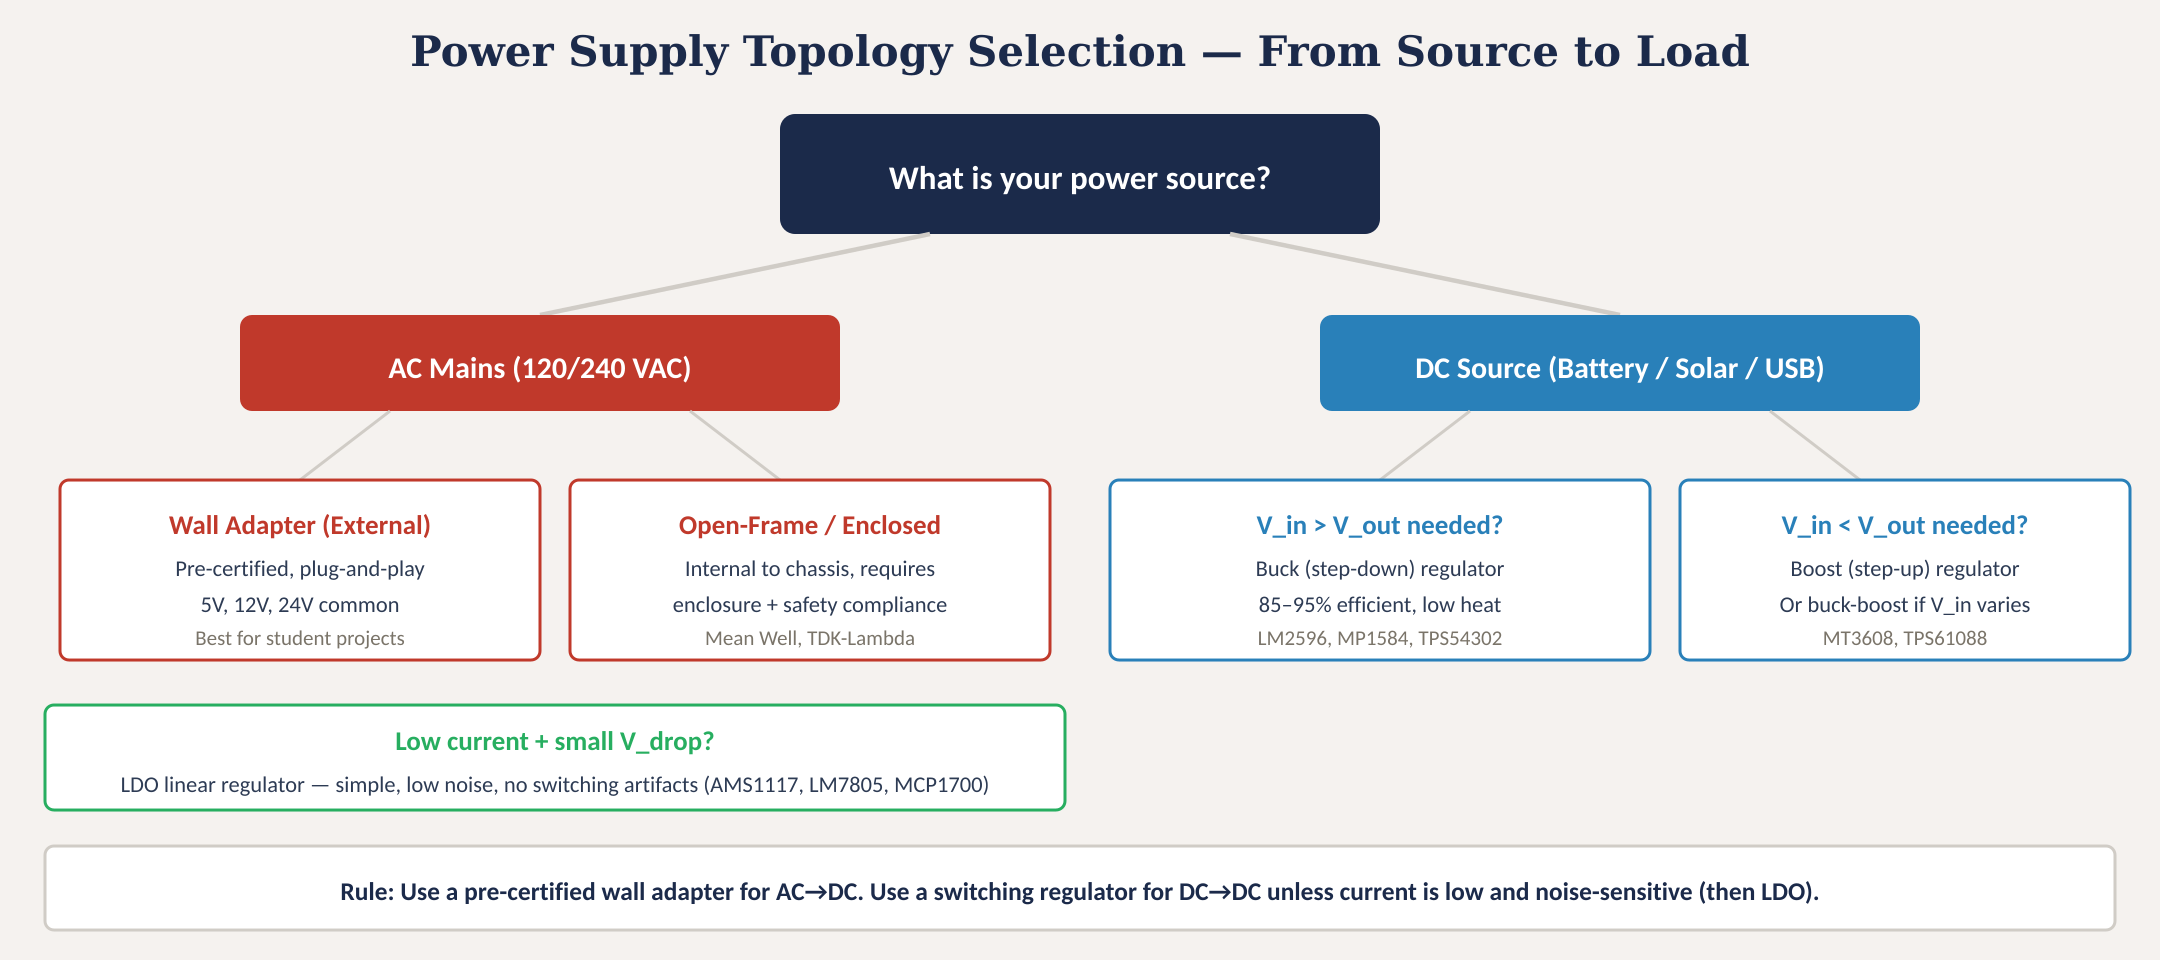
\includegraphics[width=\textwidth]{master_figs/fig_psu_topology.png}
\caption{Power supply topology decision tree, from source type through voltage conversion to specific regulator selection.}
\label{fig:psu_topology}
\end{figure}


% ══════════════════════════════════════════════════════════════════════
\section{DC Motors}
% ══════════════════════════════════════════════════════════════════════

\subsection{Motor Fundamentals}

Every DC motor operates on the Lorentz force: a current-carrying conductor in a magnetic field experiences a force. Two equations govern motor behavior:

\begin{align}
  \tau &= K_t \times I \quad \text{(torque is proportional to current)} \\
  V_{\text{back-EMF\index{back-EMF}}} &= K_e \times \omega \quad \text{(back-EMF is proportional to speed)}
\end{align}

At stall ($\omega = 0$), back-EMF is zero and current is limited only by winding resistance: $I_{\text{stall}} = V / R_{\text{winding}}$. This is typically 6--10$\times$ the rated running current and causes rapid overheating.

\subsection{Brushed DC Motors}

Simplest motor type. Mechanical commutation via carbon brushes on a copper commutator. Apply voltage, it spins; reverse polarity, it reverses. Speed control via PWM. The torque-speed curve is linear from stall torque at zero speed to no-load speed at zero torque.

\textbf{Advantages}: Cheap, simple to drive (just PWM + H-bridge\index{H-bridge}), widely available.

\textbf{Limitations}: Brush wear limits lifetime (1,000--5,000 hours), EMI from brush arcing, moderate efficiency (70--85\%).

\subsection{Brushless\index{brushless DC motor (BLDC)} DC (BLDC) Motors}

Permanent magnets on the rotor, three-phase windings on the stator. An Electronic Speed Controller (ESC) sequentially energizes the stator phases. The motor \emph{cannot function without its ESC}; they are an inseparable system.

\textbf{Advantages}: 85--95\% efficiency, 10,000+ hour life, higher power density, flat torque curve in the mid-range, lower EMI.

\textbf{Limitations}: Requires ESC (adds cost and complexity), cannot be driven directly from DC, commutation tuning matters.

\subsection{Stepper Motors}

Rotate in discrete angular steps (typically \ang{1.8} = 200 steps/rev). Open-loop positioning: count steps to know position without an encoder. NEMA 17 is the standard frame size for student projects. Driver boards (A4988, TMC2209) accept step/direction signals from any microcontroller.

\textbf{Advantages}: Precise positioning, high holding torque, no encoder needed.

\textbf{Limitations}: Torque drops rapidly with speed, runs hot (always energized), skips steps silently under overload.

\subsection{Servo Motors\index{servo motor}}

A motor + encoder + controller in a closed-loop system. Hobby servos (SG90, MG996R) are self-contained with PWM control. Industrial servos use BLDC motors with high-resolution encoders and dedicated controllers running PID loops at kHz rates.

\begin{figure}[htbp]
\centering
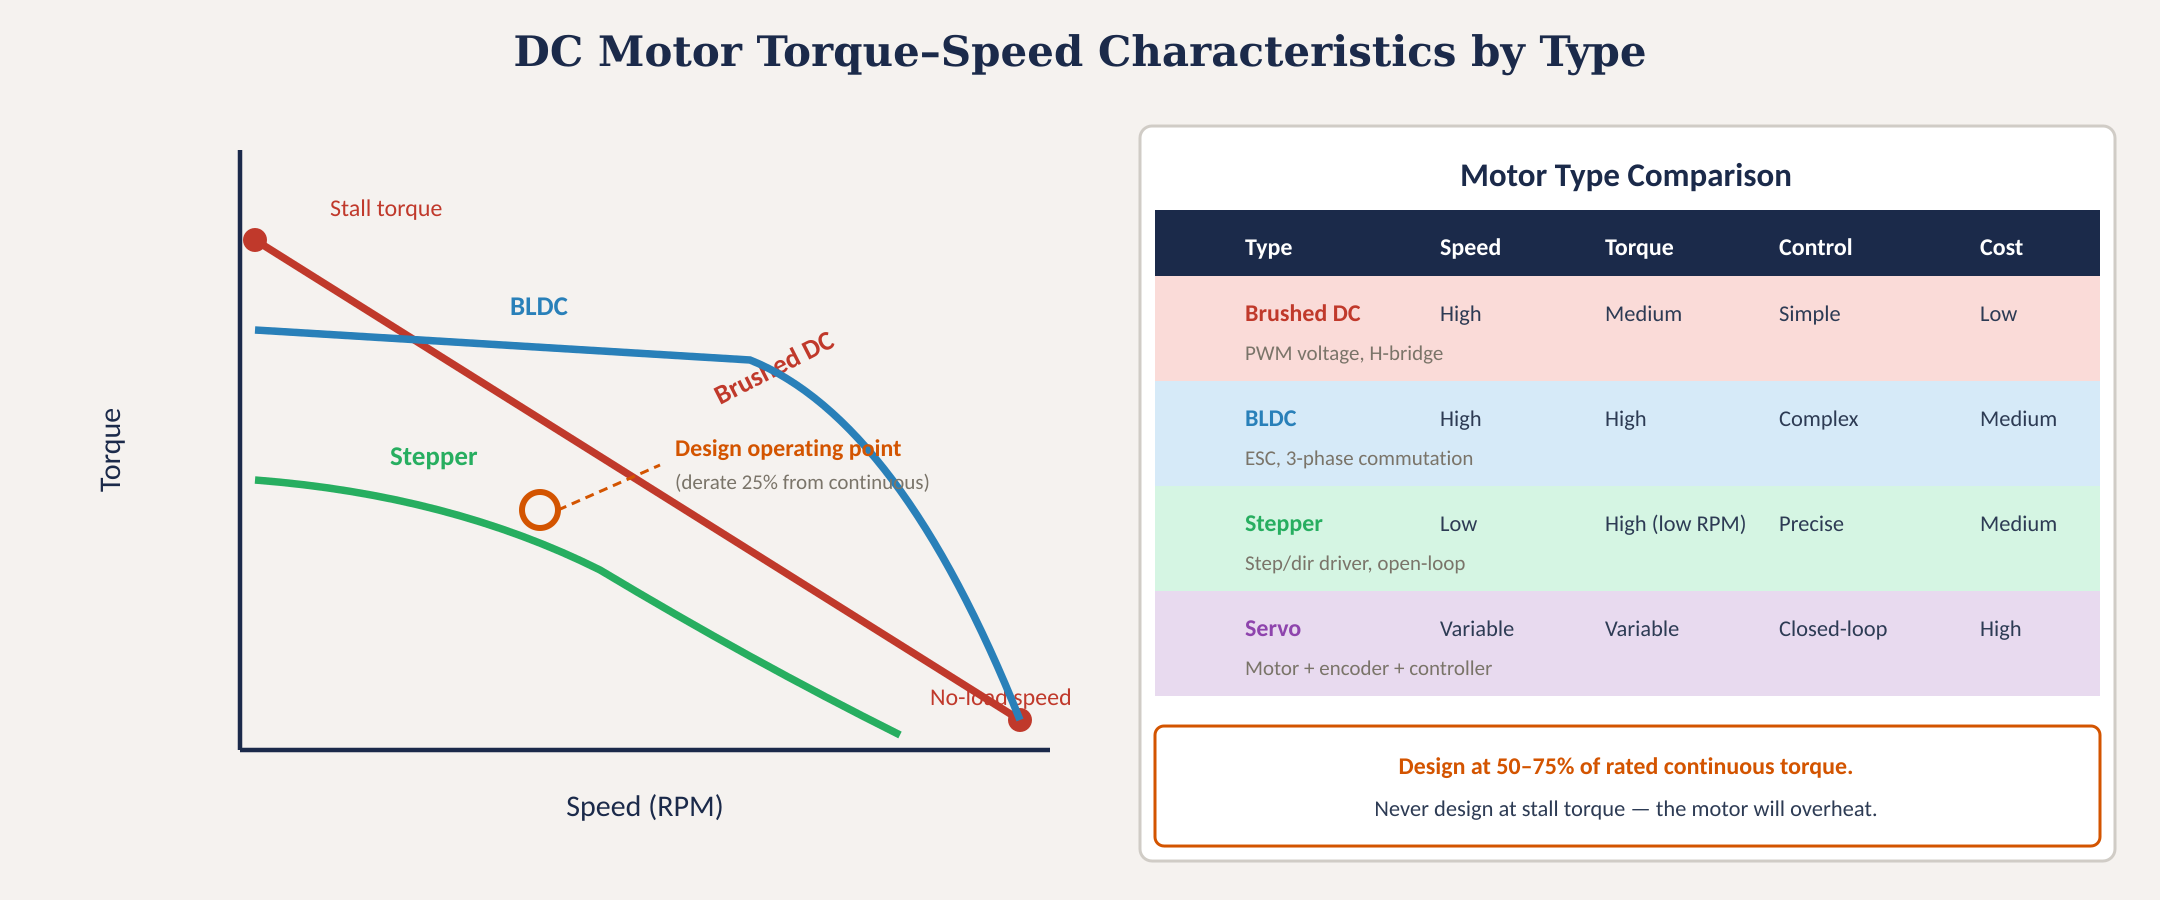
\includegraphics[width=\textwidth]{master_figs/fig_motor_curves.png}
\caption{Torque--speed characteristics for brushed DC (linear), BLDC (flat mid-range), and stepper (high-torque at low RPM) with comparison table.}
\label{fig:motor_curves}
\end{figure}

\subsection{Key Motor Specifications}

\begin{table}[htbp]
\centering\small
\begin{tabularx}{\textwidth}{l X}
  \toprule
  \textbf{Specification} & \textbf{Description} \\
  \midrule
  Rated Voltage & Nominal operating voltage. Must match your supply rail. \\
  No-Load Speed & Max speed with no load (RPM). Actual speed under load is lower. \\
  Stall Torque & Max torque at zero speed. \textbf{NOT your design point}; stall current overheats the motor. \\
  Rated / Continuous Torque & Torque the motor delivers indefinitely. Your design ceiling. Derate to 50--75\%. \\
  Rated Current & Current at rated torque. Sizes your driver and power supply. \\
  Torque Constant ($K_t$) & Torque per ampere (N$\cdot$m/A). Calculate required current: $I = \tau_{\text{load}} / K_t$. \\
  \bottomrule
\end{tabularx}
\caption{Key motor specifications.}
\end{table}

\begin{warningbox}[Never Design at Stall Torque]
Stall current = $V_{\text{rated}} / R_{\text{winding}}$, typically 6--10$\times$ the rated running current. At stall, all electrical power converts to heat in the windings. A motor will overheat and fail within seconds to minutes. Always design at 50--75\% of the \emph{continuous} rated torque.
\end{warningbox}

\subsection{Motor Drive Electronics}
\label{sec:motor_drivers}

Every motor type needs a matched driver circuit:

\begin{itemize}[leftmargin=1.5em]
  \item \textbf{H-Bridge (Brushed DC)}: Four transistors for bidirectional current. L298N (2A, legacy), BTS7960 (43A), DRV8871 (3.6A). \textbf{Must include flyback diodes\index{flyback diode}}; back-EMF from inductive loads will destroy unprotected transistors.
  \item \textbf{ESC (BLDC)}: Converts DC + throttle signal to three-phase AC. Drone ESCs are cheap and widely available. Use bidirectional or 4-quadrant ESC for reversing.
  \item \textbf{Stepper Driver}: Converts step + direction signals into motor phase currents. A4988 (2A), DRV8825 (2.5A), TMC2209 (2A, silent). \textbf{Set the current limit potentiometer before powering on.}
  \item \textbf{Servo Controller}: Hobby servos need only a PWM signal (1--2\,ms pulse, 50\,Hz). Industrial servos require dedicated controllers.
\end{itemize}


% ══════════════════════════════════════════════════════════════════════
\section{Pumps}
% ══════════════════════════════════════════════════════════════════════

\subsection{Positive Displacement vs.\ Dynamic}

\textbf{Positive displacement (PD)} pumps trap a fixed volume per cycle and force it into the discharge. Flow is proportional to speed and nearly independent of pressure. Self-priming. Pulsating flow. Types: gear, diaphragm, peristaltic, piston, vane.

\textbf{Dynamic (centrifugal)} pumps impart kinetic energy to the fluid via a spinning impeller. Flow varies with discharge pressure (follows a pump curve). Smooth, continuous flow. \emph{Not} self-priming. Best for high-volume, lower-pressure applications.

\subsection{Pump Types}

\subsubsection{Gear Pumps}
Two meshing gears trap fluid between teeth and housing. Self-priming, handles viscous fluids (oil, glycol). Constant flow rate. Used in hydraulic systems and lubrication. Primary failure mode: wear from particle contamination. Always use inline filtration.

\subsubsection{Diaphragm Pumps}
A flexible diaphragm oscillates to create suction and discharge. Seal-less design isolates fluid from moving parts. Self-priming, handles corrosive and abrasive fluids. Pulsating flow requires dampeners.

\subsubsection{Peristaltic Pumps}
Rollers compress a flexible tube, pushing fluid forward. Zero contamination risk; fluid only contacts the tube. Easy maintenance: swap the tube. Gentle on shear-sensitive fluids. Limited to $\sim$30\,psi. Tube fatigue is the primary maintenance concern.

\subsubsection{Centrifugal / Impeller Pumps}
Spinning impeller accelerates fluid radially. Smooth, high-volume flow. Requires flooded suction (not self-priming). Poor with viscous fluids. Small 12V DC impeller pumps are widely available for student cooling and circulation projects.

\begin{figure}[htbp]
\centering
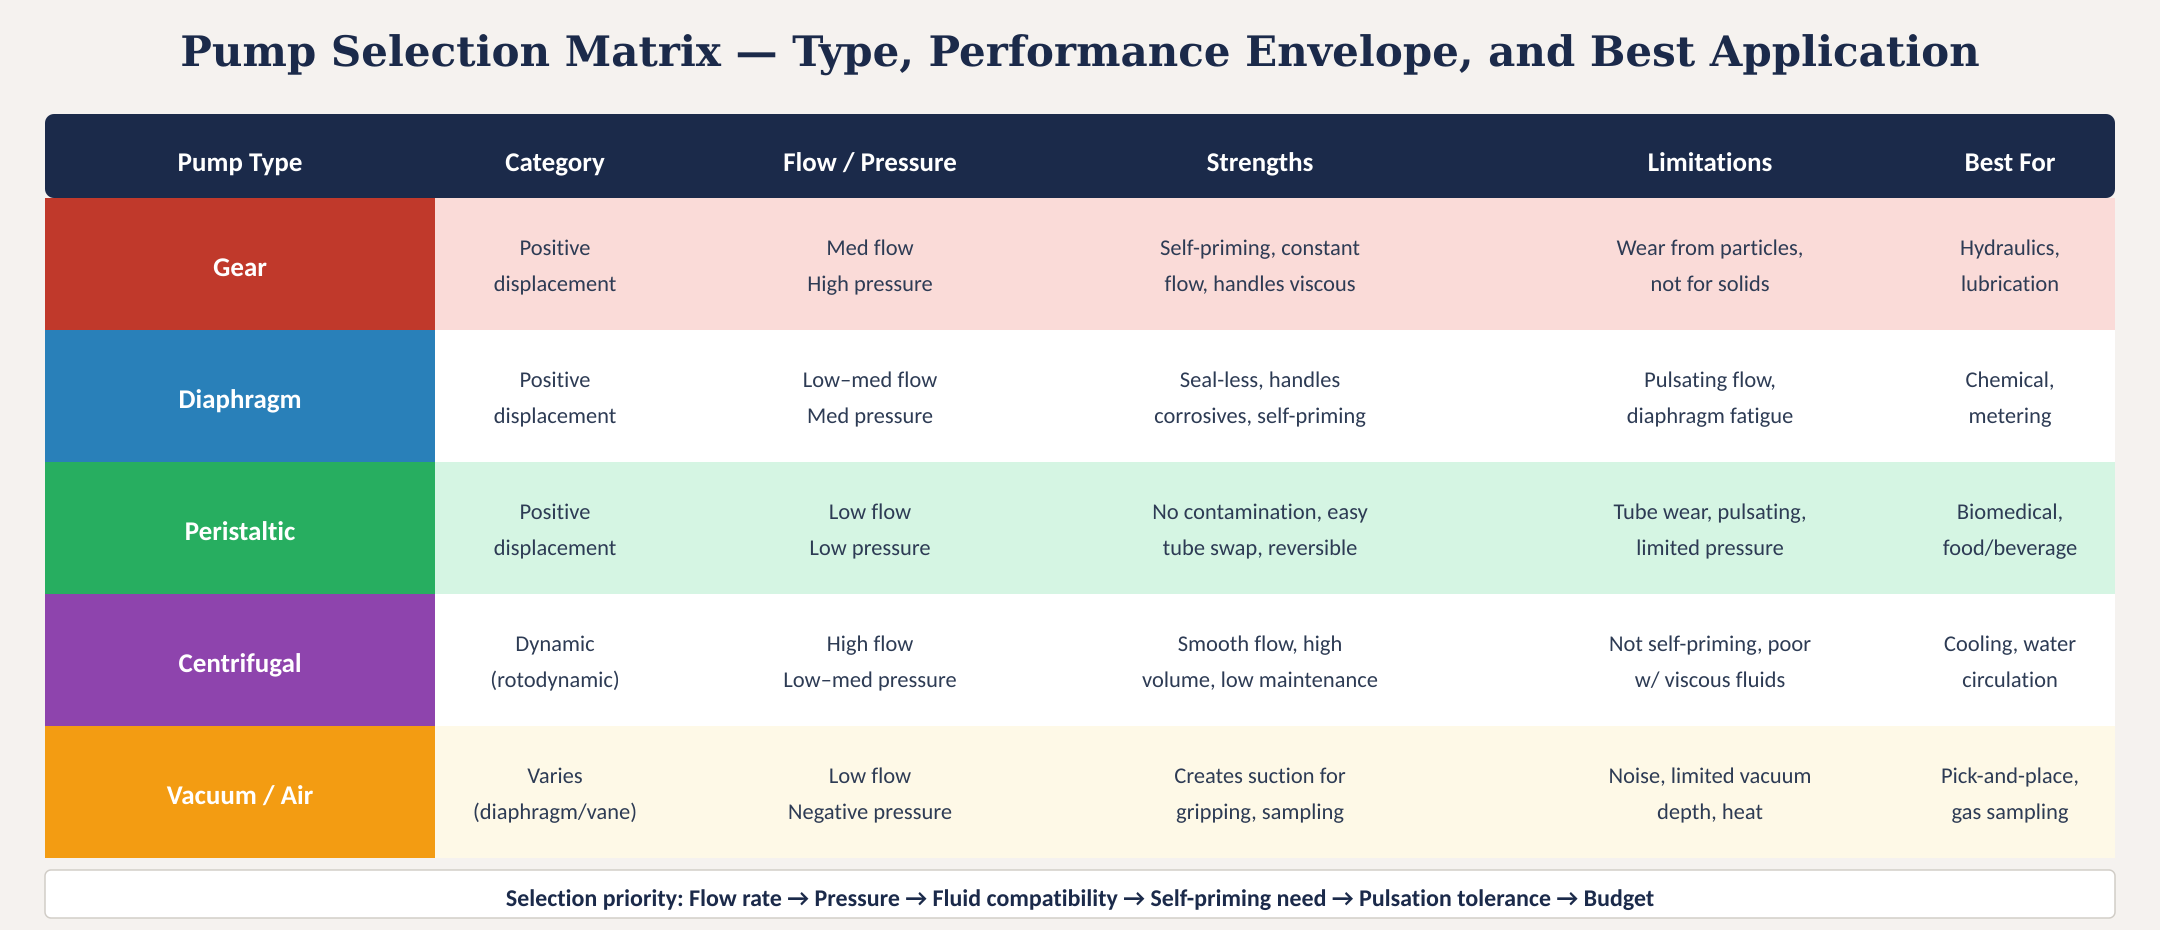
\includegraphics[width=\textwidth]{master_figs/fig_pump_matrix.png}
\caption{Pump selection matrix; type, performance envelope, strengths, limitations, and best applications.}
\label{fig:pump_matrix}
\end{figure}

\subsection{Key Pump Specifications}

\begin{table}[htbp]
\centering\small
\begin{tabularx}{\textwidth}{l X}
  \toprule
  \textbf{Specification} & \textbf{Description} \\
  \midrule
  Flow Rate & Volume per unit time (L/min, mL/min). Must meet demand with $\geq$25\% margin. \\
  Discharge Pressure / Head & Max pressure (psi/bar) or total dynamic head (ft/m). Must exceed system losses. \\
  Fluid Compatibility & Wetted materials must be compatible with the pumped fluid. Check seal charts. \\
  Self-Priming & PD pumps: yes. Centrifugal: no (must be flooded). \\
  Motor Integration & Many small pumps include integrated 12V/24V DC motors; specify the assembly. \\
  \bottomrule
\end{tabularx}
\caption{Key pump specifications.}
\end{table}


% ══════════════════════════════════════════════════════════════════════

\subsection{Worked Example: Motor Selection for a Belt Conveyor}

\textbf{Requirements}: Move 1\,kg payload at 0.1\,m/s on a horizontal belt conveyor. Belt drive with 50\,mm diameter driven roller.

\textbf{Step 1: Calculate load torque.}
Conveyor force = payload weight + belt friction = $(1.0 \times 9.81) + (1.0 \times 9.81 \times 0.3) = 12.75$\,N (assuming $\mu = 0.3$ for belt on roller).

Torque at roller = $F \times r = 12.75 \times 0.025 = 0.319$\,N$\cdot$m.

\textbf{Step 2: Calculate required speed.}
Roller angular velocity = $v/r = 0.1/0.025 = 4.0$\,rad/s = 38.2\,RPM.

\textbf{Step 3: Select motor with margin.}
Required motor torque (with 2$\times$ margin): $0.319 \times 2 = 0.638$\,N$\cdot$m at 38\,RPM. A typical NEMA~17 stepper (0.44\,N$\cdot$m rated) is insufficient. Options: (a) 12\,V DC gearmotor with 50:1 ratio (Pololu 37D: 0.8\,N$\cdot$m at 50\,RPM, \$25), or (b) NEMA~17 stepper with 5:1 planetary gearbox\index{planetary gear} (0.44 $\times$ 5 $\times$ 0.95 = 2.09\,N$\cdot$m at 40\,RPM, \$40).

\textbf{Step 4: Verify power budget\index{power budget}.}
$P = \tau \times \omega = 0.319 \times 4.0 = 1.28$\,W mechanical. At 70\% motor efficiency: $P_{electrical} = 1.28/0.70 = 1.83$\,W. At 12\,V: $I = 1.83/12 = 0.15$\,A running. Stall current (Pololu 37D): 5.5\,A. Power supply must handle 5.5\,A inrush.

\textbf{Step 5: Select driver.}
DC gearmotor: L298N H-bridge (2\,A continuous, inadequate for 5.5\,A stall). Better: BTS7960 (43\,A, \$8). Include flyback diodes (integrated in BTS7960).

\textbf{BOM entries}: Motor: Pololu 4756 (12V 50:1 37D gearmotor), \$24.95. Driver: BTS7960 module, \$7.50. Mounting: Pololu 1084 bracket, \$7.49.

\section{Selection and Design Practice}
% ══════════════════════════════════════════════════════════════════════

\subsection{Unified Selection Framework}

\begin{figure}[htbp]
\centering
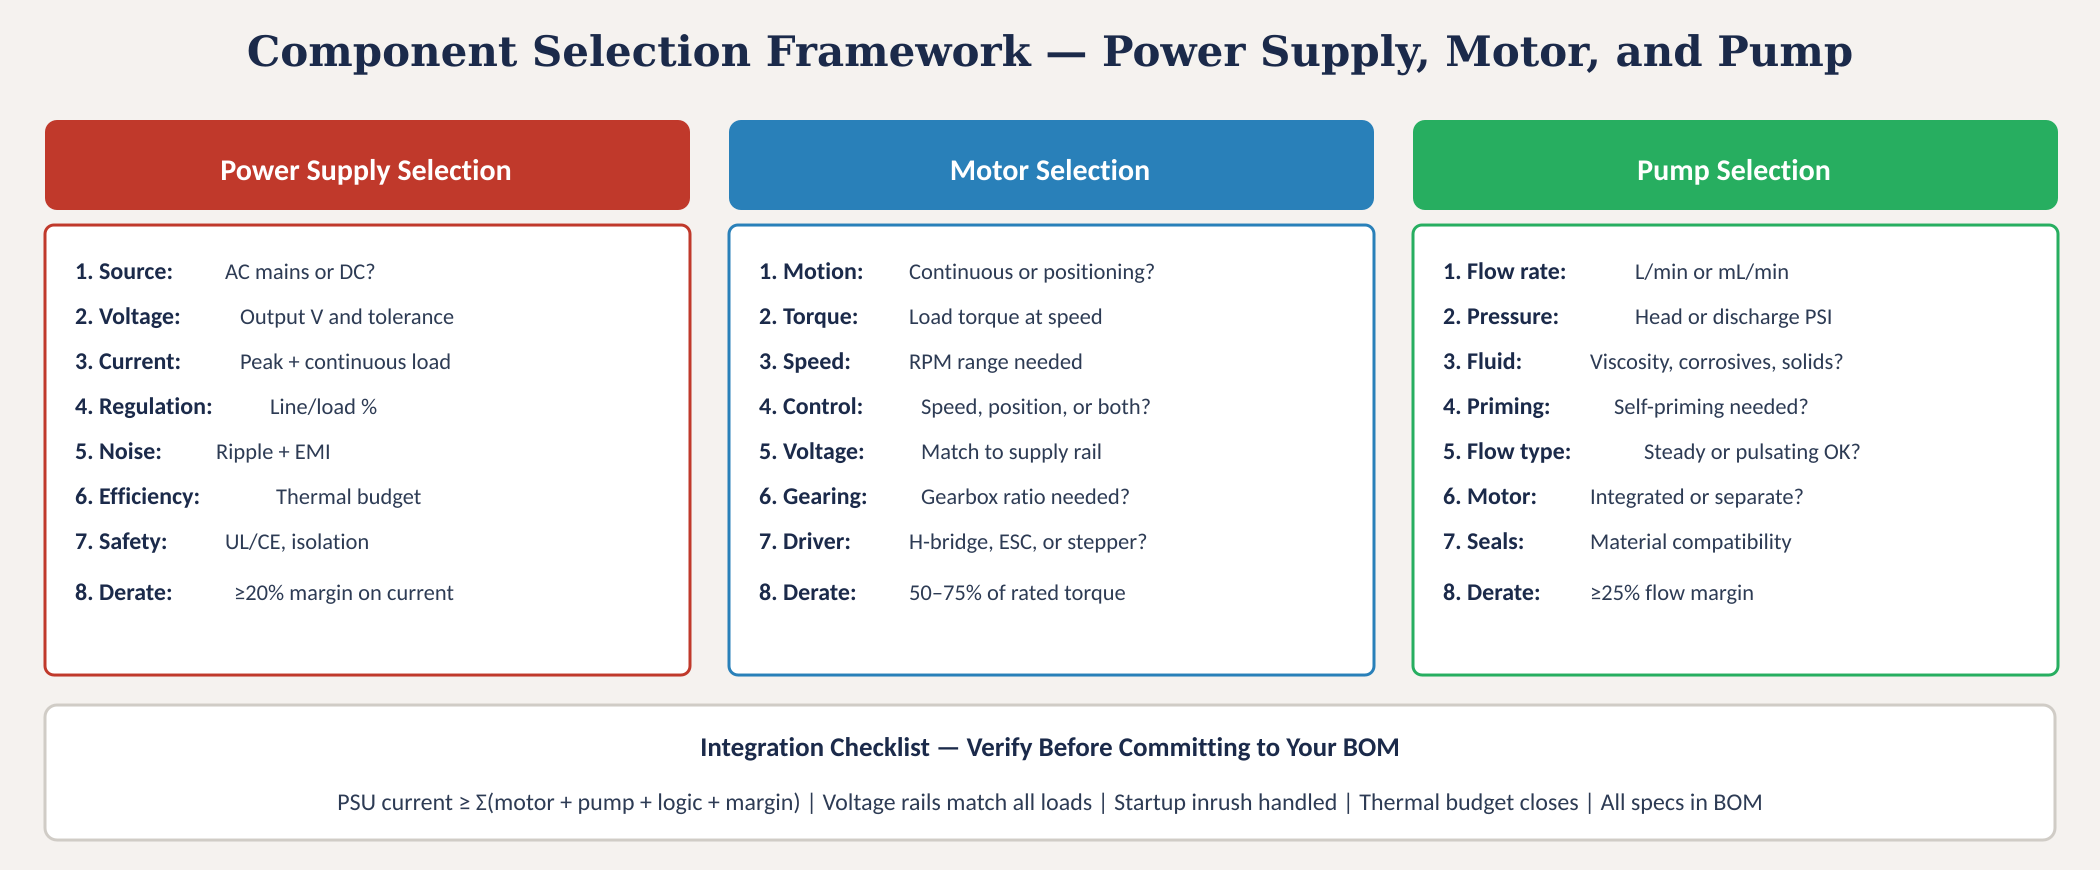
\includegraphics[width=\textwidth]{master_figs/fig_selection_framework.png}
\caption{Parallel selection flows for power supply, motor, and pump with integration verification checklist.}
\label{fig:selection_framework_b}
\end{figure}

\subsection{Design Rules}

\begin{enumerate}[leftmargin=1.5em]
  \item \textbf{Build a power budget spreadsheet first.} List every component with its voltage rail, continuous current, and peak current. Sum the columns. Add 25\% margin.
  \item \textbf{Calculate mechanical load torque before selecting a motor.} $\tau = F \times r$ for linear-to-rotary. Include friction, inertia, and acceleration torque. Select a motor with rated torque $\geq 1.5\times$ your load.
  \item \textbf{For fluid systems, map your complete flow circuit}, pipe lengths, fittings, elevation, filters, to calculate total system head loss. Select a pump whose curve crosses your system curve with margin.
  \item \textbf{Motor inrush is the \#1 power supply problem.} A motor rated at 2\,A running may draw 15\,A at startup. Size your supply for inrush, or use soft-start circuits.
  \item \textbf{Separate power and signal grounds.} Run motor power on dedicated wires back to the supply. Never share ground wires between motors and sensitive electronics.
  \item \textbf{Document everything in your BOM:} part number, manufacturer, voltage, current, torque, flow rate, and procurement source.
\end{enumerate}

\begin{keyconceptbox}[Five Key Takeaways]
\begin{enumerate}[nosep,leftmargin=1.5em]
  \item Power supplies: use pre-certified wall adapters for AC-DC; switching regulators for efficient DC-DC; LDOs only for low-current, noise-sensitive loads.
  \item Motors: match type to control need; brushed DC for simplicity, BLDC for efficiency, stepper for open-loop positioning, servo for closed-loop precision. Every motor needs a driver.
  \item Pumps: positive displacement for precise flow and self-priming; centrifugal for high-volume smooth flow. Match wetted materials to your fluid.
  \item Derating is non-negotiable: 20\% current margin on power supplies, 25--50\% torque margin on motors, 25\% flow margin on pumps.
  \item Integration: build a power budget first, size for inrush, separate power and signal grounds, document every selection in your BOM.
\end{enumerate}
\end{keyconceptbox}


% ══════════════════════════════════════════════════════════════════════
\section{Artifact Handoff: What This Chapter Supports}
\begin{table}[htbp]\centering\small
\begin{tabularx}{\textwidth}{l X l}
\toprule
\textbf{Artifact} & \textbf{Description} & \textbf{Forward Reference} \\
\midrule
Power Budget & Voltage rails, current draws, margin analysis & Ch.~9 (protection), Ch.~5 (integration) \\
Motor Selection & Torque/speed calcs, driver selection, BOM entry & Ch.~11, Ch.~16 (p.\,\pageref{ch:transmission}), BOM \\
Pump Selection & Flow/pressure calcs, wetted material verification & BOM, test plan \\
\bottomrule
\end{tabularx}
\end{table}

\section{Power Supply Noise and Its Effect on Measurement}
Every switching power supply generates output ripple at the switching frequency (typically 100\,kHz--2\,MHz) and its harmonics. This ripple propagates to every powered circuit, including sensitive analog signal conditioning.

\textbf{Ripple specification}: a ``12\,V, 5\,A'' switching supply may have 50--200\,mV peak-to-peak ripple. For a 14-bit ADC with $\pm$10\,V range (LSB $= 1.22$\,mV), 50\,mV of ripple is 41\,LSBs of noise, potentially dominating the measurement uncertainty.

\textbf{Mitigation}: (1) use a linear post-regulator (LDO) between the switching supply and the analog circuits. The LDO's PSRR (Power Supply Rejection Ratio) attenuates the ripple by 40--70\,dB. A 50\,mV ripple becomes $< 0.05$\,mV after an LDO with 60\,dB PSRR. (2) Add LC filtering: a 100\,$\mu$H inductor followed by 100\,$\mu$F capacitor provides $\sim$40\,dB attenuation at 100\,kHz. (3) Physically separate the analog and digital power paths on the PCB, connecting them only at the power entry point.

\section{Battery Selection for Portable Systems}
\textbf{Lithium Polymer (LiPo)}: 3.7\,V nominal, 4.2\,V charged, 3.0\,V discharged. Energy density: 150--250\,Wh/kg. Most common for student projects. Available in standard sizes from 500\,mAh to 10{,}000\,mAh. Requires BMS (Battery Management System) for charge control and overdischarge protection. \textbf{Never charge unattended; never charge above 4.2\,V; never discharge below 3.0\,V.}

\textbf{Lithium Iron Phosphate (LFP/LiFePO4)}: 3.2\,V nominal. Lower energy density but inherently safer (no thermal runaway). Better cycle life (2000+ vs.\ 500 for LiPo). Preferred for applications where safety is paramount.

\textbf{NiMH}: 1.2\,V nominal. Robust, safe, well-understood. Lower energy density than lithium. Good for applications where cost matters more than weight. Standard AA and AAA sizes simplify replacement.

\textbf{Runtime estimation}: runtime $= C_{\text{battery}}(\text{mAh}) / I_{\text{average}}(\text{mA})$\,hours. A 2000\,mAh battery powering a 200\,mA average load: $2000/200 = 10$\,hours. Derate by 20\% for real-world conditions (self-discharge, temperature, aging): effective runtime $\approx 8$\,hours.

\begin{quickrefbox}[Quick Reference: Common Motor/Driver Combinations]
\begin{table}[H]\centering\small
\begin{tabularx}{\linewidth}{l l c X}
\toprule
\textbf{Motor} & \textbf{Driver} & \textbf{Typical V/A} & \textbf{Notes} \\
\midrule
Pololu micro gearmotor & DRV8871 & 6--12\,V / 3.6\,A & Small robots, mechanisms \\
N20 gearmotor & TB6612FNG & 3--12\,V / 1.2\,A & Dual channel, breadboard-friendly \\
NEMA 17 stepper & A4988 or DRV8825 & 8--35\,V / 2\,A & 3D printer axes, linear stages \\
NEMA 23 stepper & TB6600 & 9--42\,V / 4\,A & CNC, heavier linear motion \\
12\,V brushed DC & BTS7960 & 5--27\,V / 43\,A & High-current, bidirectional \\
Brushless (BLDC) & ESC (hobby-grade) & 7--22\,V / varies & Drones, pumps, fans \\
Small servo (SG90) & Direct PWM from MCU & 5\,V / 0.5\,A & Position control, no driver IC \\
Large servo (MG996R) & Direct PWM + ext.\ supply & 5--7\,V / 2.5\,A stall & Separate power rail from MCU \\
\bottomrule
\end{tabularx}
\end{table}
\end{quickrefbox}

\section{Practice Questions}
% ══════════════════════════════════════════════════════════════════════

\subsection{Conceptual Questions}

\begin{enumerate}[leftmargin=1.5em]
  \item What is the fundamental difference between how a linear regulator and a switching regulator convert voltage?

\begin{keyconceptbox}[Requirements Mapping: From Motor Curves to Shall-Statements]
A motor's torque--speed curve directly generates testable requirements:
\begin{itemize}[nosep,leftmargin=1.5em]
\item ``System shall move payload at 0.5\,m/s'' $\to$ Calculate wheel RPM from diameter, verify the motor's torque at that RPM exceeds load torque with $\geq$50\% margin.
\item ``Motor runs continuously'' $\to$ MOT-REQ: Motor current at operating point shall be $\leq$75\% of continuous rated current. Calculate: $I_{req} = \tau_{load} / K_t$.
\item ``Battery life 4 hours'' $\to$ PSU-REQ: Battery capacity $\geq I_{avg} \times 4 \times 1.3$ (aging margin).
\item ``Pump delivers 2\,L/min at 10\,psi'' $\to$ PUMP-REQ: Pump shall deliver $\geq$2.5\,L/min at $\geq$12\,psi system head loss (25\% margin).
\end{itemize}
If your requirement says ``0.5\,m/s'' but the motor cannot produce the required torque at the corresponding RPM, the requirement and hardware are in conflict. The torque--speed curve resolves this \emph{before} you order parts.
\end{keyconceptbox}

  \item A 12\,V motor has a winding resistance of 0.5\,$\Omega$ and a rated current of 4\,A. What is the stall current? Why is this dangerous?

  \item Explain why a BLDC motor cannot function without an ESC, while a brushed DC motor can operate with just a battery connection.

  \item Your project needs to regulate a LiPo battery (3.0\,--4.2\,V) down to 3.3\,V. Why would a standard buck converter fail during battery discharge?

  \item Compare the self-priming capability of gear pumps versus centrifugal pumps. How does this affect installation design?

  \item Why must you include flyback diodes when driving a motor with an H-bridge? What happens without them?

  \item A power supply is rated at 10\,A at 25\,\degC{}. If your enclosure reaches 50\,\degC{}, can you still draw 10\,A? Explain.

  \item What is the primary advantage of a peristaltic pump over a gear pump for biomedical applications?
\end{enumerate}

\subsection{Application / Scenario Questions}

\begin{enumerate}[resume,leftmargin=1.5em]
  \item Your design uses a 24\,V wall adapter powering two DC motors (24\,V, 3\,A each running, 20\,A stall each) and an Arduino (5\,V, 200\,mA). Design the power architecture: what regulators are needed, what is the minimum supply current rating, and how do you handle motor inrush?

  \item You need to pump ethylene glycol coolant at 2\,L/min through a closed cooling loop with 3\,m of tubing, six fittings, and no elevation change. Which pump type do you recommend and why? What seal material?

  \item Your team selects a NEMA 17 stepper for a linear stage. The required force is 20\,N at 50\,mm/s using a 10\,mm lead screw\index{lead screw}. Calculate the required torque and verify whether a standard NEMA 17 (0.4\,N$\cdot$m rated) is adequate.

  \item \textbf{Diagnostic scenario}: Your prototype's motor operates normally when powered from a bench supply but stutters and resets the microcontroller when powered from the project's 12\,V battery pack. The battery is fully charged. What is the most likely cause, and how do you fix it?
\end{enumerate}

\subsection{Answers}

\begin{enumerate}[leftmargin=1.5em]
  \item A linear regulator dissipates excess voltage as heat (acts as a variable resistor). A switching regulator rapidly switches the input on/off and uses an inductor to transfer energy efficiently, achieving 85--95\% efficiency versus 40--80\% for linear.

  \item $I_{\text{stall}} = V/R = 12/0.5 = 24\,A$; six times the rated current. At stall, all 288\,W ($24 \times 12$) converts to heat in the windings. The motor will overheat and fail within seconds.

  \item A brushed DC motor has mechanical commutation (brushes and commutator) that automatically reverses current in the rotor windings. A BLDC motor's rotor has permanent magnets and the stator windings must be energized in a precise three-phase sequence by the ESC, which reads rotor position via Hall sensors or back-EMF sensing. Without the ESC, there is no commutation and no rotation.

  \item A buck converter requires $V_{\text{in}} > V_{\text{out}}$ to regulate. When the LiPo discharges below 3.3\,V (which happens as the cell depletes toward 3.0\,V), the buck cannot maintain the output. A buck-boost converter is required because it handles the input crossing the output voltage.

  \item Gear pumps are self-priming: they can draw fluid up from below the pump inlet by creating suction through the gear tooth spaces. Centrifugal pumps are not self-priming and require a flooded suction (pump inlet below fluid level). This means centrifugal pumps must be installed below the tank or use a foot valve and check valve to maintain prime.

  \item A motor is an inductive load. When current is suddenly switched off, the collapsing magnetic field generates a voltage spike (back-EMF) that can be many times the supply voltage. Without flyback diodes, this spike destroys the H-bridge transistors. Flyback diodes clamp the spike by providing a current path for the decaying magnetic energy.

  \item No. Every power supply has a thermal derating curve. At 50\,\degC{}, the supply has less thermal headroom to dissipate heat. A typical derating might reduce capacity to 70--80\% of the 25\,\degC{} rating, meaning 7\,--8\,A. Always check the datasheet derating curve.

  \item The fluid in a peristaltic pump only contacts the inside of a disposable tube; no seals, rotors, or metal surfaces touch the fluid. This eliminates contamination risk and allows easy sterilization by swapping the tube. A gear pump has fluid contact with gears, housing, and shaft seals, making sterilization far more difficult.

  \item Architecture: wall adapter provides 24\,V rail directly to motors via H-bridges. A buck converter (e.g., LM2596) steps 24\,V down to 5\,V for the Arduino. Minimum supply current: continuous = $2 \times 3 + 0.2 = 6.2\,A$, but inrush = $2 \times 20 = 40\,A$ simultaneously. A 10\,A supply with bulk capacitance ($\geq$4700\,$\mu$F) on the motor rail to absorb inrush, plus staggered motor startup in firmware (start one motor, wait 500\,ms, start the second), is the practical solution.

  \item A small DC centrifugal impeller pump is appropriate: the loop is closed (no priming issue if pump is at the bottom), flow is moderate, ethylene glycol is low viscosity, and smooth non-pulsating flow is preferred for cooling. Seal material: Viton (FKM) or EPDM; both compatible with ethylene glycol at moderate temperatures.

  \item Torque = force $\times$ lead / ($2\pi \times$ efficiency). $\tau = 20 \times 0.010 / (2\pi \times 0.9) = 0.035$\,N$\cdot$m. The NEMA 17 at 0.4\,N$\cdot$m rated torque provides $0.4 / 0.035 = 11.4\times$ margin. However, at the required speed: $50\text{ mm/s} / 10\text{ mm/rev} = 5\text{ rev/s} = 300\text{ RPM}$. Check the stepper's torque-speed curve at 300 RPM; torque typically drops to 40--60\% of holding torque, giving 0.16--0.24\,N$\cdot$m. Still adequate ($4.6$--$6.9\times$ margin), but verify on the actual datasheet curve.

  \item Most likely cause: the battery cannot supply the motor inrush current. Unlike a bench supply (which can deliver virtually unlimited current), a battery has internal resistance. During motor startup, the inrush current ($6$--$10\times$ running) causes a voltage drop across the battery's internal resistance, drooping the 12\,V rail. If it drops below the buck converter's minimum input or the microcontroller's brown-out threshold ($\sim$2.7\,V for most AVR/ARM), the MCU resets. Fix: add a large bulk capacitor ($\geq$4700\,$\mu$F) on the battery rail close to the motor driver, use a battery with lower internal resistance (higher C-rating), implement soft-start in firmware, and add a separate regulated supply for the MCU with adequate input capacitance.
\end{enumerate}


% ══════════════════════════════════════════════════════════════════════

